\documentclass[twoside]{book}

% Packages required by doxygen
\usepackage{calc}
\usepackage{doxygen}
\usepackage{graphicx}
\usepackage[utf8]{inputenc}
\usepackage{makeidx}
\usepackage{multicol}
\usepackage{multirow}
\usepackage{textcomp}
\usepackage[table]{xcolor}

% Font selection
\usepackage[T1]{fontenc}
\usepackage{mathptmx}
\usepackage[scaled=.90]{helvet}
\usepackage{courier}
\usepackage{amssymb}
\usepackage{sectsty}
\renewcommand{\familydefault}{\sfdefault}
\allsectionsfont{%
  \fontseries{bc}\selectfont%
  \color{darkgray}%
}
\renewcommand{\DoxyLabelFont}{%
  \fontseries{bc}\selectfont%
  \color{darkgray}%
}

% Page & text layout
\usepackage{geometry}
\geometry{%
  a4paper,%
  top=2.5cm,%
  bottom=2.5cm,%
  left=2.5cm,%
  right=2.5cm%
}
\tolerance=750
\hfuzz=15pt
\hbadness=750
\setlength{\emergencystretch}{15pt}
\setlength{\parindent}{0cm}
\setlength{\parskip}{0.2cm}
\makeatletter
\renewcommand{\paragraph}{%
  \@startsection{paragraph}{4}{0ex}{-1.0ex}{1.0ex}{%
    \normalfont\normalsize\bfseries\SS@parafont%
  }%
}
\renewcommand{\subparagraph}{%
  \@startsection{subparagraph}{5}{0ex}{-1.0ex}{1.0ex}{%
    \normalfont\normalsize\bfseries\SS@subparafont%
  }%
}
\makeatother

% Headers & footers
\usepackage{fancyhdr}
\pagestyle{fancyplain}
\fancyhead[LE]{\fancyplain{}{\bfseries\thepage}}
\fancyhead[CE]{\fancyplain{}{}}
\fancyhead[RE]{\fancyplain{}{\bfseries\leftmark}}
\fancyhead[LO]{\fancyplain{}{\bfseries\rightmark}}
\fancyhead[CO]{\fancyplain{}{}}
\fancyhead[RO]{\fancyplain{}{\bfseries\thepage}}
\fancyfoot[LE]{\fancyplain{}{}}
\fancyfoot[CE]{\fancyplain{}{}}
\fancyfoot[RE]{\fancyplain{}{\bfseries\scriptsize Generated on Tue Mar 31 2015 17\-:59\-:54 for library by Doxygen }}
\fancyfoot[LO]{\fancyplain{}{\bfseries\scriptsize Generated on Tue Mar 31 2015 17\-:59\-:54 for library by Doxygen }}
\fancyfoot[CO]{\fancyplain{}{}}
\fancyfoot[RO]{\fancyplain{}{}}
\renewcommand{\footrulewidth}{0.4pt}
\renewcommand{\chaptermark}[1]{%
  \markboth{#1}{}%
}
\renewcommand{\sectionmark}[1]{%
  \markright{\thesection\ #1}%
}

% Indices & bibliography
\usepackage{natbib}
\usepackage[titles]{tocloft}
\setcounter{tocdepth}{3}
\setcounter{secnumdepth}{5}
\makeindex

% Hyperlinks (required, but should be loaded last)
\usepackage{ifpdf}
\ifpdf
  \usepackage[pdftex,pagebackref=true]{hyperref}
\else
  \usepackage[ps2pdf,pagebackref=true]{hyperref}
\fi
\hypersetup{%
  colorlinks=true,%
  linkcolor=blue,%
  citecolor=blue,%
  unicode%
}

% Custom commands
\newcommand{\clearemptydoublepage}{%
  \newpage{\pagestyle{empty}\cleardoublepage}%
}


%===== C O N T E N T S =====

\begin{document}

% Titlepage & ToC
\hypersetup{pageanchor=false}
\pagenumbering{roman}
\begin{titlepage}
\vspace*{7cm}
\begin{center}%
{\Large library }\\
\vspace*{1cm}
{\large Generated by Doxygen 1.8.6}\\
\vspace*{0.5cm}
{\small Tue Mar 31 2015 17:59:54}\\
\end{center}
\end{titlepage}
\clearemptydoublepage
\tableofcontents
\clearemptydoublepage
\pagenumbering{arabic}
\hypersetup{pageanchor=true}

%--- Begin generated contents ---
\chapter{Library 'library'}
\label{index}\hypertarget{index}{}The main page of the documentation of your library. 
\begin{DoxyCode}
\textcolor{comment}{// You can put code in the documentation }
\end{DoxyCode}
 
\chapter{Namespace Index}
\section{Namespace List}
Here is a list of all namespaces with brief descriptions\-:\begin{DoxyCompactList}
\item\contentsline{section}{\hyperlink{namespacelib}{lib} \\*Brief description of your library namespace }{\pageref{namespacelib}}{}
\end{DoxyCompactList}

\chapter{Data Structure Index}
\section{Data Structures}
Here are the data structures with brief descriptions\-:\begin{DoxyCompactList}
\item\contentsline{section}{\hyperlink{classlib_1_1Class}{lib\-::\-Class} \\*Brief description of your class }{\pageref{classlib_1_1Class}}{}
\end{DoxyCompactList}

\chapter{File Index}
\section{File List}
Here is a list of all files with brief descriptions\-:\begin{DoxyCompactList}
\item\contentsline{section}{/home/nacho/\-Downloads/cpp-\/project-\/template/include/library/\hyperlink{Class_8hpp}{Class.\-hpp} }{\pageref{Class_8hpp}}{}
\item\contentsline{section}{/home/nacho/\-Downloads/cpp-\/project-\/template/src/\hyperlink{Class_8cpp}{Class.\-cpp} }{\pageref{Class_8cpp}}{}
\end{DoxyCompactList}

\chapter{Namespace Documentation}
\hypertarget{namespacelib}{\section{lib Namespace Reference}
\label{namespacelib}\index{lib@{lib}}
}


Brief description of your library namespace.  


\subsection*{Data Structures}
\begin{DoxyCompactItemize}
\item 
class \hyperlink{classlib_1_1Class}{Class}
\begin{DoxyCompactList}\small\item\em Brief description of your class. \end{DoxyCompactList}\end{DoxyCompactItemize}


\subsection{Detailed Description}
Brief description of your library namespace. 
\chapter{Data Structure Documentation}
\hypertarget{classlib_1_1Class}{\section{lib\-:\-:Class Class Reference}
\label{classlib_1_1Class}\index{lib\-::\-Class@{lib\-::\-Class}}
}


Brief description of your class.  




{\ttfamily \#include $<$Class.\-hpp$>$}



Collaboration diagram for lib\-:\-:Class\-:\nopagebreak
\begin{figure}[H]
\begin{center}
\leavevmode
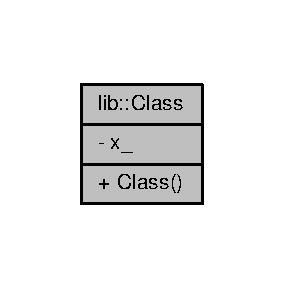
\includegraphics[width=136pt]{classlib_1_1Class__coll__graph}
\end{center}
\end{figure}
\subsection*{Public Member Functions}
\begin{DoxyCompactItemize}
\item 
\hyperlink{classlib_1_1Class_a9ac2c333cced24167c6de5d82eb8e121}{Class} (int x)
\begin{DoxyCompactList}\small\item\em Constructor of the class. \end{DoxyCompactList}\end{DoxyCompactItemize}
\subsection*{Private Attributes}
\begin{DoxyCompactItemize}
\item 
int \hyperlink{classlib_1_1Class_a3bc9070f77eddefb3970da53bc2f35cc}{x\-\_\-}
\begin{DoxyCompactList}\small\item\em Brief info of the member variable. \end{DoxyCompactList}\end{DoxyCompactItemize}


\subsection{Detailed Description}
Brief description of your class. 

Extended description. Format valid for classes and member functions. 

\subsection{Constructor \& Destructor Documentation}
\hypertarget{classlib_1_1Class_a9ac2c333cced24167c6de5d82eb8e121}{\index{lib\-::\-Class@{lib\-::\-Class}!Class@{Class}}
\index{Class@{Class}!lib::Class@{lib\-::\-Class}}
\subsubsection[{Class}]{\setlength{\rightskip}{0pt plus 5cm}lib\-::\-Class\-::\-Class (
\begin{DoxyParamCaption}
\item[{int}]{x}
\end{DoxyParamCaption}
)}}\label{classlib_1_1Class_a9ac2c333cced24167c6de5d82eb8e121}


Constructor of the class. 


\begin{DoxyParams}{Parameters}
{\em x} & Random integer \\
\hline
\end{DoxyParams}


\subsection{Field Documentation}
\hypertarget{classlib_1_1Class_a3bc9070f77eddefb3970da53bc2f35cc}{\index{lib\-::\-Class@{lib\-::\-Class}!x\-\_\-@{x\-\_\-}}
\index{x\-\_\-@{x\-\_\-}!lib::Class@{lib\-::\-Class}}
\subsubsection[{x\-\_\-}]{\setlength{\rightskip}{0pt plus 5cm}int lib\-::\-Class\-::x\-\_\-\hspace{0.3cm}{\ttfamily [private]}}}\label{classlib_1_1Class_a3bc9070f77eddefb3970da53bc2f35cc}


Brief info of the member variable. 



The documentation for this class was generated from the following files\-:\begin{DoxyCompactItemize}
\item 
/home/nacho/\-Downloads/cpp-\/project-\/template/include/library/\hyperlink{Class_8hpp}{Class.\-hpp}\item 
/home/nacho/\-Downloads/cpp-\/project-\/template/src/\hyperlink{Class_8cpp}{Class.\-cpp}\end{DoxyCompactItemize}

\chapter{File Documentation}
\hypertarget{Class_8hpp}{\section{/home/nacho/\-Downloads/cpp-\/project-\/template/include/library/\-Class.hpp File Reference}
\label{Class_8hpp}\index{/home/nacho/\-Downloads/cpp-\/project-\/template/include/library/\-Class.\-hpp@{/home/nacho/\-Downloads/cpp-\/project-\/template/include/library/\-Class.\-hpp}}
}
{\ttfamily \#include $<$iostream$>$}\\*
Include dependency graph for Class.\-hpp\-:\nopagebreak
\begin{figure}[H]
\begin{center}
\leavevmode
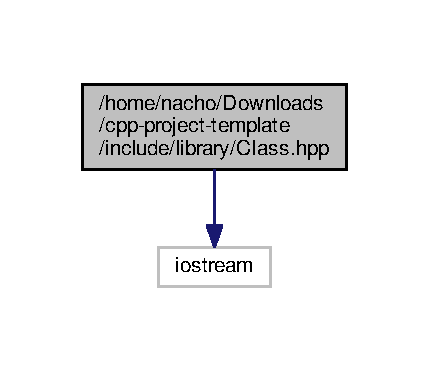
\includegraphics[width=206pt]{Class_8hpp__incl}
\end{center}
\end{figure}
This graph shows which files directly or indirectly include this file\-:\nopagebreak
\begin{figure}[H]
\begin{center}
\leavevmode
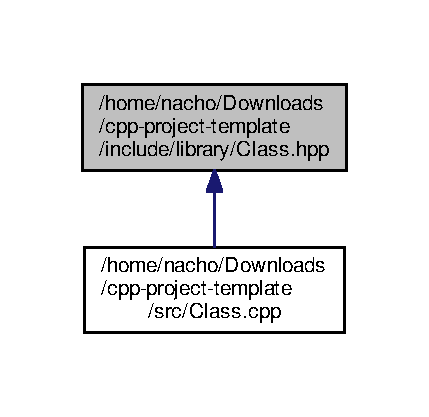
\includegraphics[width=206pt]{Class_8hpp__dep__incl}
\end{center}
\end{figure}
\subsection*{Data Structures}
\begin{DoxyCompactItemize}
\item 
class \hyperlink{classlib_1_1Class}{lib\-::\-Class}
\begin{DoxyCompactList}\small\item\em Brief description of your class. \end{DoxyCompactList}\end{DoxyCompactItemize}
\subsection*{Namespaces}
\begin{DoxyCompactItemize}
\item 
\hyperlink{namespacelib}{lib}
\begin{DoxyCompactList}\small\item\em Brief description of your library namespace. \end{DoxyCompactList}\end{DoxyCompactItemize}

\hypertarget{Class_8cpp}{\section{/home/nacho/\-Downloads/cpp-\/project-\/template/src/\-Class.cpp File Reference}
\label{Class_8cpp}\index{/home/nacho/\-Downloads/cpp-\/project-\/template/src/\-Class.\-cpp@{/home/nacho/\-Downloads/cpp-\/project-\/template/src/\-Class.\-cpp}}
}
{\ttfamily \#include \char`\"{}library/\-Class.\-hpp\char`\"{}}\\*
Include dependency graph for Class.\-cpp\-:\nopagebreak
\begin{figure}[H]
\begin{center}
\leavevmode
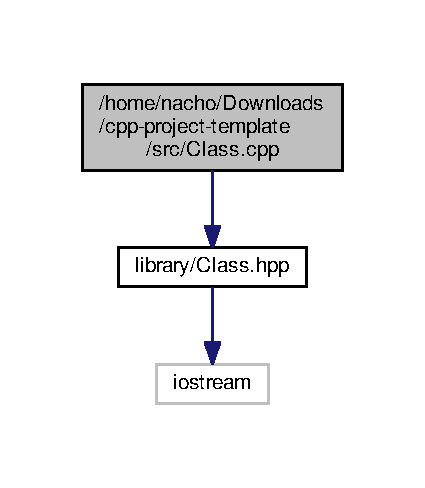
\includegraphics[width=204pt]{Class_8cpp__incl}
\end{center}
\end{figure}
\subsection*{Namespaces}
\begin{DoxyCompactItemize}
\item 
\hyperlink{namespacelib}{lib}
\begin{DoxyCompactList}\small\item\em Brief description of your library namespace. \end{DoxyCompactList}\end{DoxyCompactItemize}

%--- End generated contents ---

% Index
\newpage
\phantomsection
\addcontentsline{toc}{chapter}{Index}
\printindex

\end{document}
